\documentclass[11pt]{article}
\usepackage{amsmath}
%\usepackage{extsizes}
\usepackage{amsmath,amssymb}
%\usepackage{omegavn,ocmrvn}
%\usepackage[utf8x]{inputenc}
\usepackage[utf8]{vietnam}

\usepackage{listings}
\lstset{language=Python}          % Set your language (you can change the language for each code-block optionally)


\usepackage{longtable}
\usepackage{answers}
\usepackage{graphicx}
\usepackage{array}
\usepackage{pifont}
\usepackage{picinpar}
\usepackage{enumerate}
\usepackage[top=3.0cm, bottom=3.5cm, left=3.5cm, right=2.5cm] {geometry}

\usepackage{extarrows}
\usepackage{hyperref}


\newtheorem{bt}{Câu}
\newcommand{\RR}{\mathbb R}
\Newassociation{sol}{Solution}{ans}
\newtheorem{ex}{Câu}
\renewcommand{\solutionstyle}[1]{\textbf{ #1}.}


\begin{document}
% \noindent

\begin{tabular*}
	{\linewidth}{c>{\centering\hspace{0pt}} p{.7\textwidth}}
	Trường ĐHKHTN, ĐHQGHN & {\bf Học Kỳ 2 (2021-2022)}
	\tabularnewline
	K64 TTƯD - Thầy Hà Phi & {\bf Bài Tập Giải Tích Số \\ \today}
	% Exercises on pages 239, 240 Cheney/Kincaid are really nice
	\tabularnewline
	\rule{1in}{1pt}  \small  & \rule{2in}{1pt} %(Due date:)
	\tabularnewline
	%  \tabularnewline
	%  &(Đề thi có 1 trang)
\end{tabular*}




\begin{center}
	{\bf Bài Tiểu Luận - Tính Toán Khoa Học}
\end{center}

Các em có thể dùng MATLAB để hỗ trợ cho việc tính toán nhanh gọn, ví dụ để tìm phân tích Kalman của hệ.

\begin{bt}
Hãy đọc và dịch phần đóng khung trong các trang 48-50 để hiểu về mô hình giảm xóc được sử dụng trong ô tô. Sau đó chuyển các hệ $(2.10)-(2.11)$ về dạng bậc nhất với biến điều khiển đầu vào $r$ bằng việc giới thiệu thêm các biến mới để biểu diễn $\dot{x}$, $\dot{y}$.  
Chú ý lập bảng liệt kê giá trị của các tham số $k_w$, $k_s$, ...
\end{bt}

\begin{bt}
a) Đối với hệ điều khiển bậc nhất vừa tìm được, hãy nghiên cứu xem hệ đó có điều khiển được không, có quan sát được không? \\
b) Xác định số biến điều khiển được và số biến không điều khiển được của hệ. \\
c) Xác định số biến quan sát được và số biến không quan sát được của hệ. \\
d) Hãy tìm phân tích Kalman của hệ, từ đó suy ra nhận dạng tối thiểu của hệ. 
\end{bt}

\begin{bt}
Hàm truyền của hệ điều khiển này có thể tìm được bằng 2 cách tiếp cận: (1) Sử dụng công thức hàm truyền của hệ bậc nhất (2) sử dụng biến đổi Laplace bằng cách thay $s$ cho đạo hàm $d/dt$ như trong phần đóng khung của trang 50. Ở đây $1.31e06$ có nghĩa là $1.31 * 10^6$. \\
a) Hãy tìm dạng chính tắc điều khiển được sao cho hàm truyền của nó có dạng $(2.13)$. \\
b) Hãy tìm dạng chính tắc quan sát được sao cho hàm truyền của nó có dạng $(2.13)$. 
\end{bt}

\begin{bt}
Hãy chuyển hệ liên tục về hệ rời rạc bằng cách lấy mẫu với thời gian lấy mẫu là $T = 1$. Từ đó nghiên cứu tính điều khiển được và quan sát được của hệ rời rạc.
\end{bt}

\begin{bt}
Cho LMI sau với các biến số là ma trận $W$ bất kỳ, các ma trận $X$ và $Y$ là đối xứng, xác định dương
%
\begin{equation}
	\m{XA^T + AX + BW + W^TB^T+ Y & A_d X \\ XA^T_d & -Y} < 0,
\end{equation}
%
trong đó $A = \m{-1 & 0 & 1 \\ 0 & 2 & -1 \\ 2 & 0 & -3}$, $A_d = \m{ 1 & 0 & 1 \\ 2 & 1 & 1 \\ 0  & 0 & -1}$, $B = \m{1 & 1 \\ 1 & 2 \\ 0 & 1}$.
\end{bt}
%Đáp số thầy giải ra là 
%
%\begin{figure}
%	\centering
%	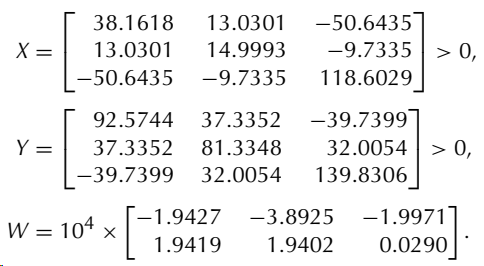
\includegraphics[width=0.7\linewidth]{screenshot001}
%	\caption{}
%	\label{fig:screenshot001}
%\end{figure}

\end{document}



